% 本原稿用の条件マクロ
%章ごとにコンパイルできるようにするための設定.
%このマクロが定義されていない場合,チャプター内は個別のTEXソースとして扱われる.
\expandafter\ifx\csname MasterFile\endcsname\relax
\documentclass[a4j,twoside,12pt, dvipdfmx]{thesis} % 修論・卒論など (ページが右端にでる) 
\usepackage{amsmath, amssymb}
\usepackage{mysettings}
\usepackage{graphicx}
\usepackage{color}
\usepackage{comment}

\begin{document}

\addtocounter{chapter}{+2}

\setlength{\baselineskip}{1.95zw}
\setlength{\textheight}{30\baselineskip}
\mainmatter

\fi
% これより上は削除しちゃダメ
% 本原稿用の条件マクロここまで
%
%\newcommand{\argmax}{\mathop{\rm arg~max}\limits}
\renewcommand\thefootnote{\arabic{footnote})}
\def\vector#1{\mbox{\boldmath $#1$}}

\chapter{提案手法}\label{meth}
% ここに本文
本章では,提案手法について説明する.本研究は大きく分けて以下の 4 つに分類される.
\begin{enumerate}
  \item 文からのグラフ作成
  \item ノードの特徴量畳込み
  \item グラフを表現する埋め込み生成
  \item グラフ間の類似度の評価
\end{enumerate}
それぞれの方法について2種類の手法を採用し, 計16種類の手法で比較を行った. \par
モデルの概要を図\ref{fig:ModelFlow}に示す.
\begin{figure}
  \centering
  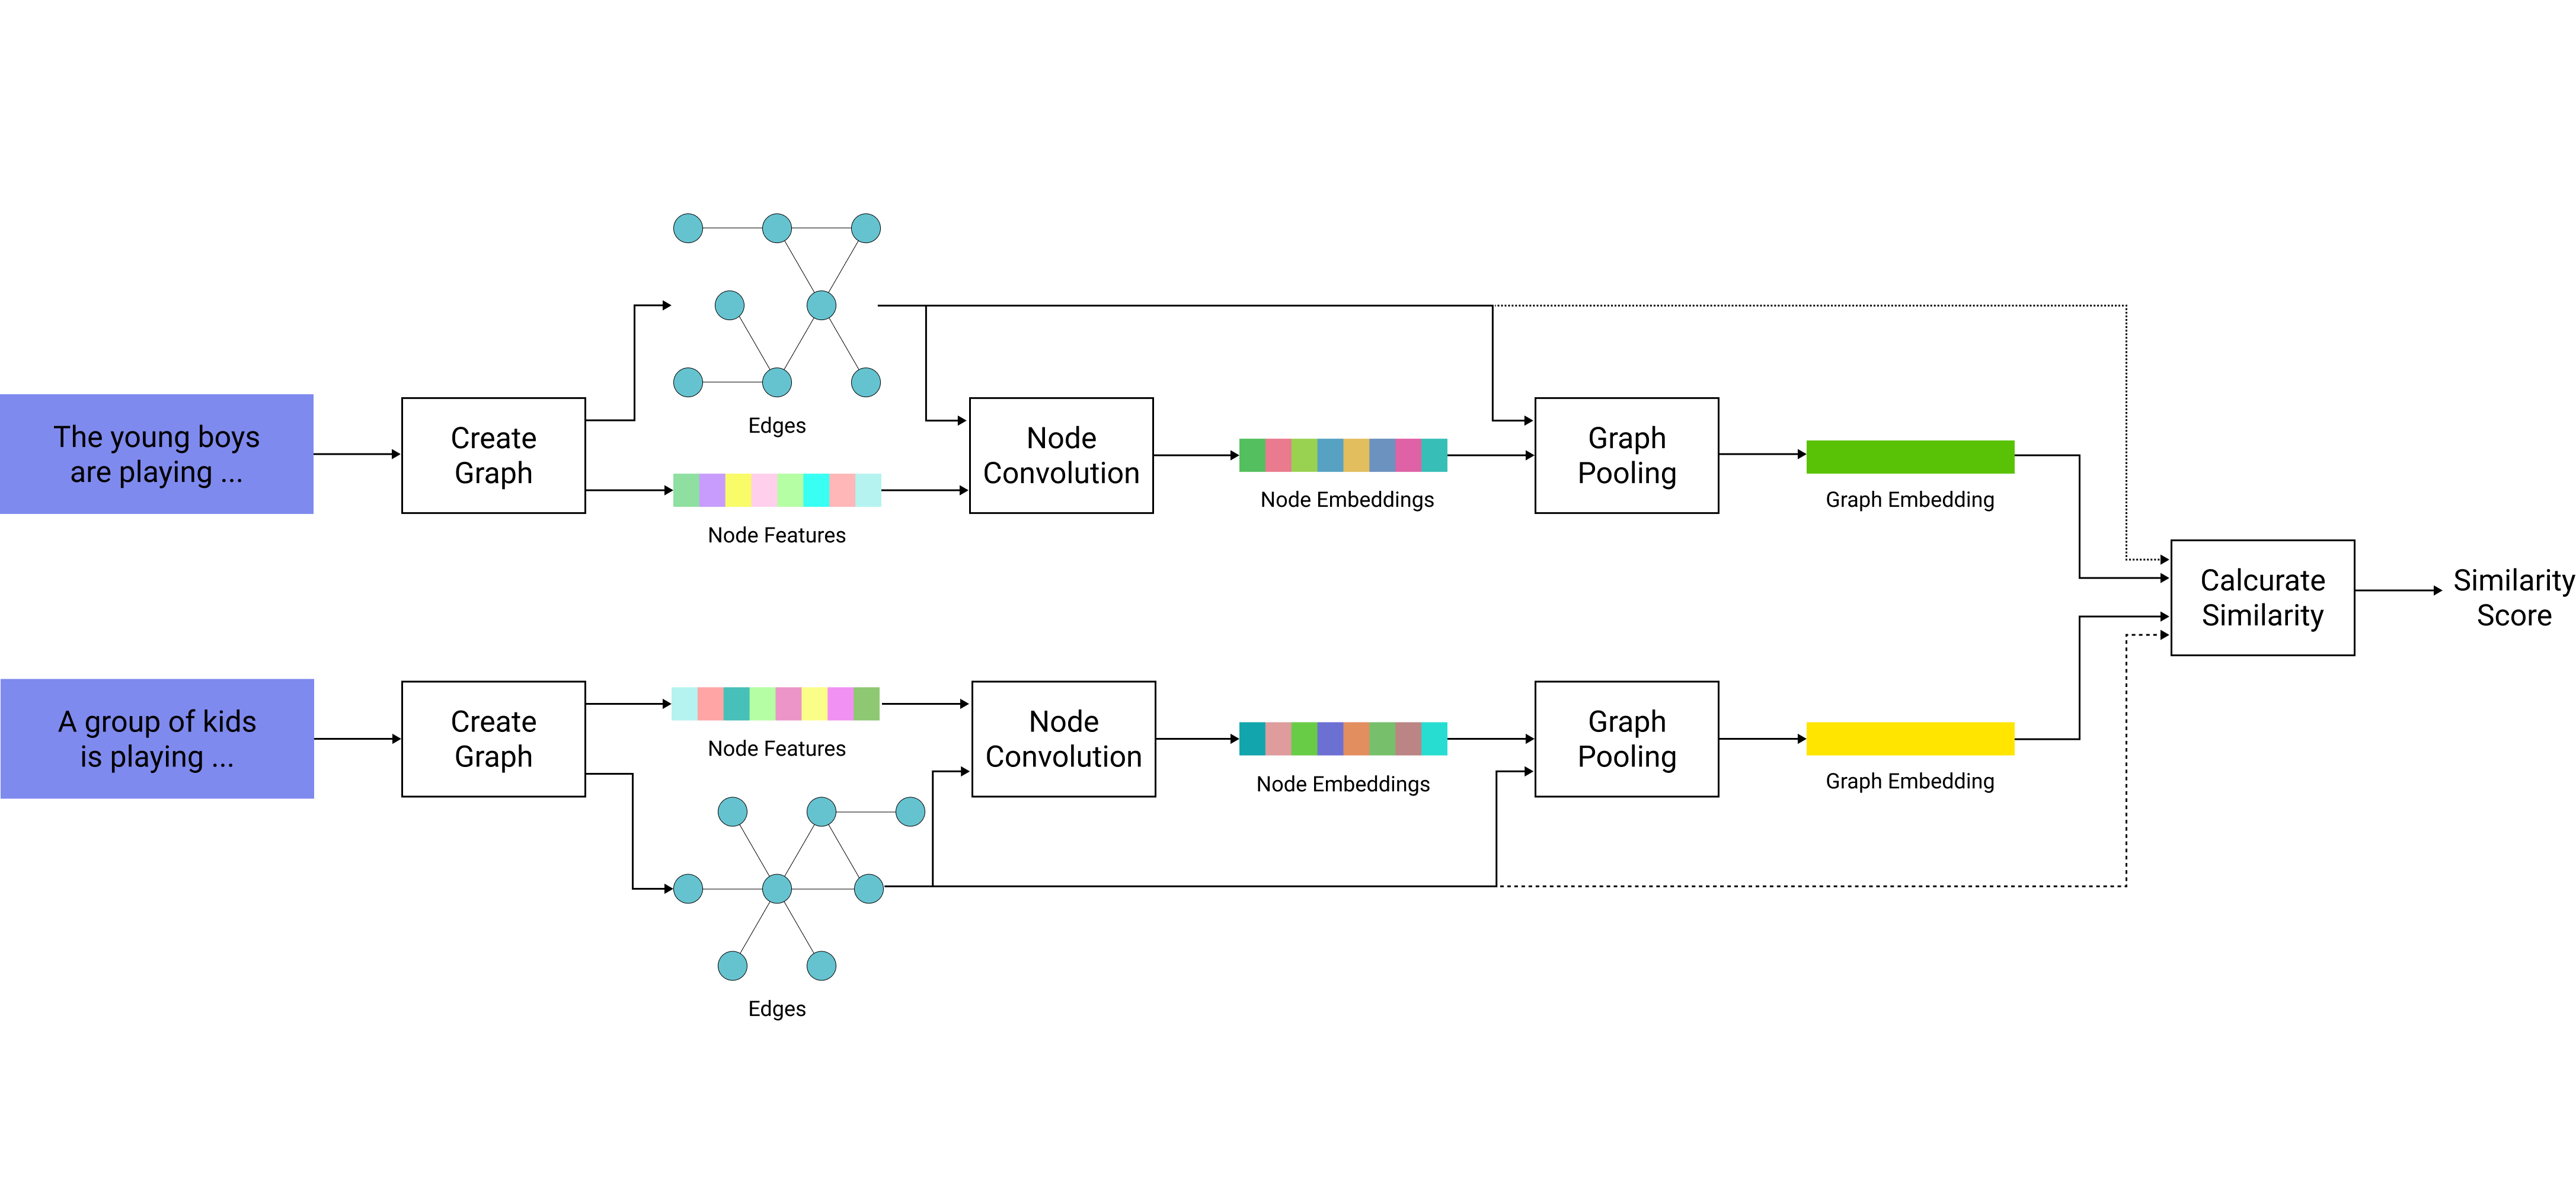
\includegraphics[width=\linewidth]
  {img/ModelFlow.jpg}
  \caption{モデルの概要}
  \label{fig:ModelFlow}
\end{figure}

\ref{meth:createGraph}節では文からのグラフ作成,\ref{meth:convNode}節ではノード畳込み \ref{meth:createEmbedding}節ではグラフを表現する埋め込み生成, \ref{meth:calculateSimilarity}節ではグラフ間の類似度計算について述べる.

\section{文からのグラフ作成}\label{meth:createGraph}
本節では,文からのグラフ生成手法について説明する.\
グラフの生成について,以下の2つを行う.
\begin{enumerate}
  \item ノード生成
  \item エッジ生成
\end{enumerate}
また, 本研究では以下の2通りのエッジ生成方法を元に, 2 種類のグラフを生成し実験した.
\begin{enumerate}
  \item 依存関係に基づくエッジ生成
  \item 依存関係と隣接関係に基づくエッジ生成
\end{enumerate}

\subsection{ノード生成}\label{meth:createNode}
文からのグラフの生成において,各ノードはそれぞれの単語とし,その単語のレンマの埋め込みを取得し,ノードの特徴量とする.

\subsection{エッジ生成}\label{meth:createEdge}
エッジの生成には2通りの方法を用いた.
\subsubsection{依存関係に基づくエッジ生成}
各エッジの生成には Universal Dependencies に基づく構文解析を行い,単語間に依存関係があれば双方向にエッジを作成し,無向グラフを生成した.

\subsubsection{依存関係と隣接関係に基づくエッジ生成}
依存関係に基づくエッジ生成に加えて, 単語間に隣接関係があれば双方向エッジを作成し,無向グラフを生成した.

\section{ノードの特徴量畳込み}\label{meth:convNode}
本節では, ノードの特徴量畳込み手法について説明する.
ノードの特徴量畳み込みでは2通りの方法を採用した.
\subsection{Graph Convolutional Network (GCN)}
この方法では,ノードの畳み込みにKipf ら\cite{kipf2017semi}と同様の Graph Convolutional Network (GCN) を用いる.
GCN の第$l$層における出力は式\ref{eq:methGCN}で表される.
\begin{equation}
  \label{eq:methGCN}
  H^{(l)}=f(\tilde{D}^{-\frac{1}{2}}\tilde{A}\tilde{D}^{-\frac{1}{2}}H^{(l-1)}W_{1}^{(l-1)})
\end{equation}
ここで,$\tilde{A} = A + I_{N}$はノード自身へのエッジを追加した無向グラフの隣接行列であり,$I_N$は単位行列である.
$\tilde{D}_{ii} = \sum_{j} \tilde{A}_{ij}$であり,$W_{1}^{(l)}$は層に応じた学習可能な重み行列,$f(\cdot)$は$ReLU(\cdot) = \max (0, \cdot)$のような活性化関数である.
また,$H^{(0)}=X$となる.

\subsubsection{GraphSAGE}
この方法では, ノードの畳み込みにGraphSAGE\cite{hamilton2017inductive}を用いる.
aggregatorには, MeanAggregatorを用いる.
Mean aggregatorを用いた場合, ノード$v$に対するGraphSAGEの第$l$層の出力は式\ref{eq:methGraphSAGE}で表される.
\begin{equation}
  \label{eq:methGraphSAGE}
  h_{v}^{l} \leftarrow \sigma(\mathbf{W_{2}} \cdot \mathrm{MEAN} (\{ \mathbf{h}_{v}^{l-1}\} \cup \{ \mathbf{h}_{u}^{l-1} , \forall u \in \mathcal{N}(v) \}))
\end{equation}
ここで, $\mathbf{h}_{v}^{l}$は第$l$層でのノード$v$の埋め込みであり, $\mathbf{W_{2}}$は学習可能な重み行列, $\mathcal{N}(v)$はノード$v$の近傍ノード郡である.

\section{グラフを表現する埋め込み生成}\label{meth:createEmbedding}
本節では,グラフを表現する埋め込み生成手法について説明する.
グラフを表現する埋め込み生成では2通りの方法を採用した.
これらの方法では, 前節の方法で得られたノードレベルの埋め込みを元にグラフを表現する埋め込みを生成する.

\subsection{アテンションモジュール}
この方法は SimGNN\cite{bai2019simgnn}で用いられているアテンションモジュールと同様のものである.
アテンションモジュールから出力される, グラフを表現する埋め込み$h$は以下の式で表される.
\begin{equation}
  h = \sum_{n=1}^{N}\sigma(u_{n}^\mathsf{T}c)u_{n}= \sum_{n=1}^{N}\sigma(u_{n}^\mathsf{T} \tanh (\frac{1}{N}W_{2}\sum_{m=1}^{N}u_{m}))u_{n}
\end{equation}
ここで, $u_{n}$ はノード$n$の埋め込み, $\sigma$ はシグモイド関数, $N$はノード数, $W_{2}$は学習可能な重み行列である.

\subsection{SAGPool}
この方法では, グラフを表現する埋め込み生成にSelf-Attention Graph Pooling (SAGPool) \cite{lee2019self} を用いる.
各ノードの重要度を式\ref{eq:methAtt} で算出し, 重要度が最も高いノードの表現からグラフを表現する埋め込みを取得する.
\begin{equation}
  \label{eq:methAtt}
  Z = \sigma (\tilde{D}^{-\frac{1}{2}}\tilde{A}\tilde{D}^{-\frac{1}{2}}X\Theta_{att})
\end{equation}
ここで, $\tilde{A} = A + I_{N}$はノード自身へのエッジを追加した無向グラフの隣接行列であり,$I_N$は単位行列である.
$\tilde{D}_{ii} = \sum_{j} \tilde{A}_{ij}$であり$\Theta_{att}$はSAGPool層のパラメータである.

\section{グラフ間の類似度計算}\label{meth:calculateSimilarity}
本節では, グラフ間の類似度計算手法について説明する.
グラフ間の類似度計算では2通りの方法を採用した.
これらの方法では, 前節の方法で得られたグラフを表現する埋め込みから類似度を計算する.

\subsection{ニューラルテンソルネットワーク}
この方法は SimGNN で用いられている ニューラルテンソルネットワーク と同様のものである.
2 つのグラフの埋め込み$h_{i}$, $h_{j}$を ニューラルテンソルネットワーク に与えた出力は式\ref{eq:NTN}である.
\begin{equation} \label{eq:NTN} g(h_{i}, h_{j})=f(h_{i}^\mathsf{T}W_{3}^{[1:K]}h_{j} + V \begin{bmatrix} h_{i}\\h_{j} \end{bmatrix} + b)\end{equation}
を用いる.
ここで,$W_{3}^{[1:K]} \in R^{D \times D \times K}$は重み行列,$\begin{bmatrix} $ $ \end{bmatrix}$は結合操作,$V \in \mathbb{R}^{K\times2D}$は重みベクトル.
$b \in \mathbb{R}^{K}$はバイアスベクトル, $f(\cdot)$は$ReLU(\cdot) = \max (0, \cdot)$のような活性化関数である.得られた出力を 2 層の全結合層に与えることで, 最終的な類似度を得る.

\subsection{コサイン類似度}
この方法はコサイン類似度を用いてグラフ間の類似度計算を行うものである.
2 つのグラフの埋め込み$h_{i}$, $h_{j}$のコサイン類似度は,式\ref{eq:cos}で表される.
\begin{equation}
  \label{eq:cos}
  \cos(h_{i}, h_{j}) = \dfrac{h_{i} \cdot h_{j}}{|h_{i} | | h_{j}|}
\end{equation}

% 本原稿用の条件マクロ
% これ以降は削除しちゃダメ
\expandafter\ifx\csname MasterFile\endcsname\relax
\def\MasterFile{本原稿です}

% 参考文献
%% 本原稿用の条件マクロ
%章ごとにコンパイルできるようにするための設定.
%このマクロが定義されていない場合,チャプター内は個別のTEXソースとして扱われる.
\expandafter\ifx\csname MasterFile\endcsname\relax
\documentclass[a4j,12pt]{thesis} % 修論・卒論など (ページが右端にでる)   
\usepackage{mysettings}
\usepackage{url}

\begin{document}

\setlength{\baselineskip}{1.95zw}
\setlength{\textheight}{30\baselineskip}
\backmatter

\fi
% これより上は削除しちゃダメ
% 本原稿用の条件マクロここまで

%参考文献

\bibliographystyle{junsrt}
\bibliography{thesisB}

\clearpage


% 本原稿用の条件マクロ
% これ以降は削除しちゃダメ
\expandafter\ifx\csname MasterFile\endcsname\relax
\def\MasterFile{本原稿です}
\end{document}
\fi
% 本原稿用の条件マクロここまで


\bibliographystyle{junsrt}
\bibliography{thesisB}

\end{document}
\fi
% 本原稿用の条件マクロここまで
